\documentclass[11pt]{article}
% ============================================================================
% JASA-structured rewrite of the MWQTM manuscript.
% Main paper: model -> identification -> orthogonal inference -> concise
% simulations -> application. All audit/sensitivity/proof material is in
% supplement.tex. The original (full) draft is preserved in the MWQTM repo.
% ============================================================================
\usepackage[margin=1in]{geometry}
\usepackage{amsmath,amssymb,amsthm,bm,booktabs,graphicx,natbib,hyperref}
\hypersetup{colorlinks=true,linkcolor=blue,citecolor=blue,urlcolor=blue}
\newcommand{\editnote}[1]{\par\noindent\fbox{\parbox{0.97\linewidth}{\small\itshape #1}}\par\medskip}
\newtheorem{theorem}{Theorem}
\newtheorem{proposition}{Proposition}
\newtheorem{lemma}{Lemma}
\newtheorem{assumption}{Assumption}
\newtheorem{corollary}{Corollary}
\newcommand{\E}{\mathbb{E}}
\newcommand{\PR}{\mathbb{P}}
\newcommand{\Pn}{\mathbb{P}_n}
\newcommand{\X}{\bm{X}}
\newcommand{\bbeta}{\bm{\beta}}
\newcommand{\indc}[1]{\mathbf{1}\{#1\}}
\newcommand{\given}{\,\vert\,}
\DeclareMathOperator*{\argmin}{arg\,min}
\DeclareMathOperator*{\argmax}{arg\,max}

\title{\bf Event-aligned conditional quantile trajectories of a biomarker
before disease onset under left truncation and competing death}
\author{\thanks{}}
\date{\today}

\begin{document}
\maketitle

\begin{abstract}
Biomarkers measured before the onset of a disease are observed only under delayed
entry, loss to follow-up, competing death, and irregular visit times, and existing
event-aligned models describe only their conditional \emph{mean}. We introduce an
event-aligned conditional \emph{quantile} trajectory model: indexing time by both
the visit age and the onset age, the conditional $\tau$-quantile of the
log-biomarker among individuals who develop disease is a smooth bivariate baseline
surface plus a quantile-specific covariate effect $\bbeta_{\tau}$. The estimand is
identified from complete-event subjects without modeling the onset-time
distribution and without a censoring model. Estimation solves an event-aligned
check-function objective with a tensor-spline sieve for the baseline surface; we
show that the resulting score is implicitly density-weighted and Neyman-orthogonal
to the trajectory surface and the censoring nuisance, and we give a cross-fitted
one-step estimator with $\sqrt n$ asymptotic normality and a clustered sandwich
variance. Simulations confirm valid inference and recover non-parallel quantile
trajectories; a comparison against the conditional-mean estimator of
\citet{sun2025semiparametric} shows that the quantile model recovers distributional
heterogeneity and induced non-proportional mean contrasts that a scalar mean
coefficient collapses. We illustrate the method on cortical-thickness trajectories
before amyloid positivity.
\end{abstract}

\noindent\textbf{Keywords:} conditional quantile regression; delayed entry;
event alignment; Neyman orthogonality; sieve estimation; two time scales.

% ============================================================================
\section{Introduction}\label{sec:intro}

Disease-relevant biomarkers often change in the years before a clinical landmark,
and a central question is how that pre-onset trajectory depends on covariates.
Cohorts that follow such biomarkers are subject to several sampling features at
once: participants enter the study at staggered ages (delayed entry / left
truncation), are lost to follow-up (right censoring), may die before developing
the disease (competing risk), and are measured at irregular visit times. A useful
descriptive target aligns each trajectory to the individual's own onset age and
asks how the biomarker behaves as a function of both the visit age $u$ and the
onset age $t$. \citet{sun2025semiparametric} formalized this two-time-scale view
for the conditional \emph{mean} of the marker and developed a semiparametric
estimator under exactly these sampling complications.

The conditional mean, however, describes only the first moment. A covariate can
leave the mean trajectory unchanged while shifting the \emph{dispersion} of the
marker, or it can act only in the \emph{upper tail} of the distribution---changes
that are clinically meaningful (e.g.\ a risk allele that accelerates decline only
among the already-vulnerable) yet invisible to a mean model. More subtly, when a
covariate's effect varies across quantile levels, the \emph{induced} mean contrast
need not be proportional across $(u,t)$, so a single mean coefficient becomes a
hard-to-interpret average. These are precisely the situations a conditional
quantile model is designed to reveal.

We therefore model the entire family of conditional quantiles. Writing
$L^0(u)=\log Y^0(u)$ for the log-biomarker at visit age $u$ and $T^0$ for the
onset age, we posit, for each $\tau\in(0,1)$,
\begin{equation}
Q_\tau\!\left\{L^0(u)\given T^0=t,\,D^0\ge t,\,\X^0\right\}
   = m_{\tau,0}(u,t)+\bbeta_{\tau,0}^\top\X^0 ,
\label{eq:quantile-model}
\end{equation}
where $m_{\tau,0}$ is a smooth bivariate baseline surface over the two time scales
and $\bbeta_{\tau,0}$ is a quantile-specific covariate effect. The mean model of
\citet{sun2025semiparametric} is the analogue at the level of the first moment;
\eqref{eq:quantile-model} recovers $\tau$-varying covariate effects and, through
them, distributional features the mean cannot express.

\paragraph{Contributions.} (i) We define an event-aligned conditional quantile
estimand~\eqref{eq:quantile-model} for the disease-developing subpopulation and
give its identification from observed data under left truncation, right censoring,
competing death, and irregular visits, conditioning on the observed onset age so
that \emph{no} onset-time model is required (Section~\ref{sec:model}). (ii) We
estimate \eqref{eq:quantile-model} by a complete-event sieve check-function
objective and show that joint sieve quantile regression \emph{implicitly} carries
a density-weighted projection that makes the covariate score Neyman-orthogonal to
the trajectory surface, and that the conditional-quantile restriction makes the
score orthogonal to the censoring nuisance---so the default estimator needs no
censoring model for identification (Section~\ref{sec:est}). (iii) We give a
cross-fitted one-step estimator with $\sqrt n$ asymptotic normality and a
clustered sandwich variance, and position the practical joint-sieve estimator
relative to it (Section~\ref{sec:theory}). (iv) Simulations establish valid
finite-sample inference and, against the \emph{actual} estimator of
\citet{sun2025semiparametric}, show that the quantile model recovers dispersion
effects, non-proportional induced mean contrasts, and tail-specific effects that
a scalar mean coefficient collapses (Section~\ref{sec:sim}); an application to
pre-amyloid cortical thickness illustrates the analysis (Section~\ref{sec:app}).
Proofs, algorithms, and extensive sensitivity studies are in the Supplement.

% ============================================================================
\section{Event-aligned quantile trajectory model}\label{sec:model}

\paragraph{Target population and estimand.}
Time is age relative to a fixed origin. Let $T^0$ and $D^0$ be the ages at disease
onset and death ($T^0=\infty$ if disease-free at death); the target population is
the disease-developing subpopulation $\{D^0\ge T^0\}$. The estimand is the family
$\{m_{\tau,0}(\cdot,\cdot),\bbeta_{\tau,0}\}_{\tau\in(0,1)}$ of
\eqref{eq:quantile-model}: the conditional $\tau$-quantile of $L^0(u)=\log Y^0(u)$
given onset age $T^0=t$ and covariates $\X^0$, among individuals free of disease at
the origin who develop disease. The covariate vector $\X^0$ contains no intercept
and no deterministic function of $(u,t)$ (these are absorbed into $m_{\tau,0}$,
which would otherwise break identifiability of $\bbeta_{\tau,0}$). With the
quantile score $\psi_\tau(r)=\tau-\indc{r\le0}$, \eqref{eq:quantile-model} is the
conditional moment
\begin{equation}
\E\!\left[\psi_\tau\{L^0(u)-m_{\tau,0}(u,t)-\bbeta_{\tau,0}^\top\X^0\}
   \given T^0=t,\,D^0\ge t,\,\X^0\right]=0 .
\label{eq:moment}
\end{equation}

\paragraph{Observed data.}
Let $A^0$ be the age at study entry (delayed entry: $A^0$ may be negative).
Subjects are retained only if $\max(A^0,0)\le\min(T^0,D^0)$ (left truncation). Let
$C$ be the time from entry to loss to follow-up; follow-up ends at age $A^0+C$.
Define $Z=\min(T^0,D^0,A^0+C)$, $\Delta^T=\indc{T^0\le D^0,\,T^0\le A^0+C}$,
$\Delta^D=\indc{D^0<T^0,\,D^0\le A^0+C}$, $\Delta^C=\indc{A^0+C<\min(T^0,D^0)}$, and
$W=T^0-A^0$ when $\Delta^T=1$. The biomarker is observed at irregular pre-onset
visit ages $U_{i\ell}\in(0,T_i)$, $\ell=0,\dots,m_i$. Observed data are
$\{(\X_i,A_i,Z_i,\Delta_i^T,\Delta_i^D,\{U_{i\ell},L_{i\ell}\}_\ell)\}_{i=1}^n$.

\begin{assumption}[Conditionally independent truncation]\label{as:trunc}
$A^0\perp\{Y^0(\cdot),T^0,D^0\}\given\X^0$, with positivity
$\PR(A^0\le u\given T^0=t,D^0\ge t,\X^0=\bm x)>c_A>0$ on the estimable region.
\end{assumption}
\begin{assumption}[Independent loss to follow-up]\label{as:cens}
$C\perp\{Y^0(\cdot),T^0,D^0,N^{V,0}(\cdot)\}\given(A^0,\X^0)$, where $N^{V,0}$ is the
latent visit process.
\end{assumption}
\begin{assumption}[Noninformative visits]\label{as:visit}
$N^{V,0}(\cdot)\perp\{Y^0(\cdot),T^0,D^0\}\given(A^0,\X^0)$.
\end{assumption}

These are process-level (not pointwise) independence statements; they are what the
orthogonality argument of Section~\ref{sec:theory} uses, since they keep
$\PR(C\ge T-A\given A,\X,\{U_\ell\})=G_{C,0}(T-A\given A,\X)$ even after
conditioning on the realized visit schedule.

\begin{proposition}[Identification]\label{prop:id}
Under Assumption~\ref{as:trunc}, on the estimable region where
$\PR(A^0\le u\given T^0=t,D^0\ge t,\X^0)>c_A$, the onset-conditioned quantile in the
retained, complete-event sample equals the target $m_{\tau,0}(u,t)+\bbeta_{\tau,0}^\top\X^0$.
Death before onset ($\Delta^D=1$) places a subject outside the estimand and is
handled by conditioning, not weighting; under Assumptions~\ref{as:cens}--\ref{as:visit}
neither a censoring model nor a visit-intensity weight is needed for identification.
\end{proposition}

\noindent The proof (Supplement~A) verifies that conditioning on $(T^0=t,\X^0)$ and the
entry constraint removes the truncation selection, and that censoring and visits
alter only the design density over the $(u,t)$ plane, not the conditional quantile.
This is the formal sense in which the model needs no nuisance model of the
sampling mechanism to be identified; weights enter later only as an efficiency or
design-standardization choice.

% ============================================================================
\section{Estimation and orthogonal inference}\label{sec:est}

\subsection{Complete-event sieve quantile estimator}\label{sec:sieve}
Let $\{B_k(u,t)\}_{k=1}^K$ be a tensor-product B-spline basis over the two time
scales. Only complete-event subjects ($\Delta_i^T=1$, for whom $T_i=Z_i$ and the
basis $B(U_{i\ell},T_i)$ is computable) and their pre-onset visits contribute. For
a bounded positive observed-event weight $\omega(T,A,\X)$,
\begin{equation}
(\widehat{\bm\gamma}_{\tau,\omega},\widehat\bbeta_{\tau,\omega})
 =\argmin_{\bm\gamma,\bbeta}\ \frac1n\!\!\sum_{i:\Delta_i^T=1}\!\!\omega_i
   \sum_{\ell:0<U_{i\ell}<T_i}\!\!
   \rho_\tau\!\left(L_{i\ell}-B(U_{i\ell},T_i)^\top\bm\gamma-\X_i^\top\bbeta\right)
   +\tfrac{\lambda_n}2\bm\gamma^\top P\bm\gamma ,
\label{eq:joint}
\end{equation}
with $\rho_\tau(r)=r\{\tau-\indc{r<0}\}$ and $\widehat m_{\tau,\omega}=B^\top
\widehat{\bm\gamma}_{\tau,\omega}$. \textbf{The default is the complete-event
weight $\omega\equiv1$}, which estimates no censoring model. The
inverse-probability-of-censoring weight $\omega=1/\widehat G_C(W\given A,\X)$,
with $\widehat G_C$ from a Cox model on the time-since-entry scale, is a
design-standardization \emph{sensitivity} variant that reweights the observed-onset
sample to a prespecified design; by Proposition~\ref{prop:id} both weights target
the same $(m_{\tau,0},\bbeta_{\tau,0})$. No onset-time model is used: we condition
directly on the observed $T_i$.

\subsection{Implicit density-weighted orthogonalization}\label{sec:orth}
The first-order conditions of \eqref{eq:joint} leave the $\X$-block score
$\Pn\,\omega\X\,\psi_\tau(\widehat\varepsilon)=0$ \emph{uncentered}. The curvature
of the objective, however, is the density-weighted Gram matrix with entries
$f_{i\ell,\tau}(0)=f_{\varepsilon_\tau\given U,T,\X}(0\given U_{i\ell},T_i,\X_i)$.
Profiling out $\bm\gamma$ from the linearized conditions yields, with
$S_\lambda=D-C^\top A_\lambda^{-1}C$ the profiled information,
\begin{equation}
S_\lambda(\widehat\bbeta_\tau-\bbeta_{\tau,0})
 =\frac1n\sum_{i,\ell}\omega_i\{\X_i-g_{\tau,K,\lambda}(U_{i\ell},T_i)\}
   \psi_\tau(\varepsilon_{i\ell,\tau})+\text{bias}+R_n,
\label{eq:profiled}
\end{equation}
where $g_{\tau,K,\lambda}=C^\top A_\lambda^{-1}B$. As $\lambda_n\to0$ and the sieve
grows, $g_{\tau,K,\lambda}\to g_{\tau,0}=d\mu_\tau/d\nu_\tau$, the
density-weighted projection of $\X$ onto the trajectory surface (the
Radon--Nikodym derivative of the visit occupation measures
$\mu_\tau,\nu_\tau$ weighted by $\omega f_\tau(0)$). The projected score
$\{\X-g_{\tau,0}\}\psi_\tau(\varepsilon)$ is therefore Neyman-orthogonal to
$m_\tau$: \emph{joint sieve quantile regression performs the orthogonalization
implicitly}. The two approximation biases in \eqref{eq:profiled} (penalty and
sieve) must be $o(n^{-1/2})$ for a centered limit; they bite first at extreme
$\tau$, where $f_\tau(0)$ is small.

\subsection{Orthogonality to censoring, and a cross-fitted one-step}\label{sec:onestep}
Plugging in $\widehat G_C$ would normally add a first-order term; it does not here.
With $\xi_{i,\tau}=\sum_\ell\{\X_i-g_{\tau,0}(U_{i\ell},T_i)\}\psi_\tau(\varepsilon_{i\ell,\tau})$,
the conditional-quantile restriction and Assumption~\ref{as:visit} give
$\E[\xi_{i,\tau}\given T,A,\X,D\ge T,\{U_\ell\}]=0$, while the censoring
perturbation is a function of $(T,A,\X)$; by the tower property the censoring
derivative vanishes (Lemma~\ref{lem:orth}). The plug-in $\widehat G_C$ then enters
only through second-order products. As an explicit debiasing/validation device we
estimate the sparsity $\widehat f_\tau(0)$ by quantile spacings and the projection
$\widehat g_{\tau,\omega}$ by a density-weighted spline regression, and form a
\emph{cross-fitted} one-step estimator: with subject folds $I_1,\dots,I_{\mathcal K}$,
fit all nuisances and an initial $\widehat\bbeta^{(-k)}$ off fold $k$ and aggregate
the held-out, bread-corrected scores,
\begin{equation}
\widetilde\bbeta^{\rm CF}_{\tau,\omega}
 =\sum_{k}\frac{n_k}{n}\Big[\widehat\bbeta^{(-k)}_{\tau,\omega}
 +\widehat S_k^{-1}\,\widehat U_{\tau,\omega,k}\Big],\qquad
\widehat U_{\tau,\omega,k}=\frac1{n_k}\sum_{i\in I_k}\widehat\phi_i^{(-k)} .
\label{eq:bos-cf}
\end{equation}
Subject-level resampling preserves the within-subject clustering for inference;
fold-discipline details are in Supplement~B.

% ============================================================================
\section{Large-sample theory}\label{sec:theory}

For a generic admissible weight $\omega$ (oracle nuisances), the subject-level
influence function and information are
\[
\phi^0_{i,\tau,\omega}=\Delta_i^T\omega_i\sum_\ell\{\X_i-g_{\tau,\omega}(U_{i\ell},T_i)\}
  \psi_\tau(\varepsilon_{i\ell,\tau}),\quad
S_{\tau,\omega}=\E\Big[\indc{T\le D}r_\omega\!\sum_\ell f_\tau(0)\{\X-g_{\tau,\omega}\}^{\otimes2}\Big],
\]
with design weight $r_\omega=G_{C,0}\omega$. The complete-event default
($\omega\equiv1$) uses $r_\omega=G_{C,0}$ and contains no $\widehat G_C$; the IPCW
instance ($\omega=1/G_{C,0}$) gives $r_\omega=1$.

\begin{lemma}[Censoring orthogonality]\label{lem:orth}
Under Assumptions~\ref{as:cens}--\ref{as:visit} and \eqref{eq:quantile-model}, the
pathwise derivative of the moment in the censoring nuisance vanishes for every
admissible perturbation; hence $\widehat G_C$ contributes no first-order term and
enters only through second-order products $O_p(r_G(r_m+r_\beta))$. This is a local
orthogonality property induced by the conditional moment restriction; it is not a
double-robustness claim.
\end{lemma}

\begin{proposition}[Design-weight invariance]\label{prop:invariance}
For any bounded positive weight $w(T,A,\X)$ with $0<c_w\le w\le C_w$ on the
estimable support and nonsingular weighted information, $w\equiv1$ and
$w=1/G_{C,0}$ identify the same $(m_{\tau,0},\bbeta_{\tau,0})$; $w$ affects only
efficiency and the finite-sieve pseudo-true value. The projection and information
are weight-specific, $g_{\tau,w}=d\mu_w/d\nu_w$, so in general
$g_{\tau,\rm CC}\neq g_{\tau,\rm IPCW}$.
\end{proposition}

\begin{theorem}[Cross-fitted one-step asymptotic normality]\label{thm:main}
Fix $\tau\in(0,1)$ and an admissible weight $\omega$. Assume the observed-data
quantile restriction; $S_{\tau,\omega}$ nonsingular and
$\E\|\phi^0_{i,\tau,\omega}\|^{2+\delta}<\infty$; $f_{\varepsilon_\tau\given U,T,\X}(0)\in[c_f,C_f]$
locally Lipschitz at $0$; $\mathcal K$ fixed folds with $\min_k n_k/n\ge c_K>0$;
the fold-uniform product-rate condition
\[
\max_k\big[r_{g,k}(r_{m,k}+r_{\beta,k})+r_{\omega,k}(r_{m,k}+r_{\beta,k})
   +(r_{m,k}+r_{\beta,k})^2\big]=o_p(n^{-1/2});
\]
and fold-uniform score and bread consistency. Then the cross-fitted one-step
estimator~\eqref{eq:bos-cf} satisfies
\[
\sqrt n(\widetilde\bbeta^{\rm CF}_{\tau,\omega}-\bbeta_{\tau,0})
 =S_{\tau,\omega}^{-1}\frac1{\sqrt n}\sum_{i=1}^n\phi^0_{i,\tau,\omega}+o_p(1)
 \ \Rightarrow\ \mathcal N(0,\Sigma_{\tau,\omega}),\quad
\Sigma_{\tau,\omega}=S_{\tau,\omega}^{-1}\E(\phi^0_{i,\tau,\omega}\phi^{0\top}_{i,\tau,\omega})S_{\tau,\omega}^{-\top},
\]
with the variance subject-clustered. The default complete-event ($\omega\equiv1$)
and IPCW ($\omega=1/G_{C,0}$) instances are both root-$n$ for the same
$\bbeta_{\tau,0}$, with no censoring-correction term (Lemma~\ref{lem:orth}).
\end{theorem}

\paragraph{Practical inference.} Theorem~\ref{thm:main} is the formal inferential
route, attached to the cross-fitted one-step estimator (denoted B-OS-CF). In
applications we report the joint-sieve point estimator of \eqref{eq:joint}
(denoted A-CV; complexity chosen by subject-level cross-validation) with a
full-pipeline subject bootstrap, and use B-OS-CF as an orthogonal
validation/sensitivity estimator. A complete root-$n$ theory for the
cross-validated joint estimator (a joint-sieve Bahadur expansion with random,
CV-selected complexity) is not pursued here; the simulations of
Section~\ref{sec:sim} show that the two estimators agree closely in bias and
coverage, so the bootstrap inference reported for A-CV is empirically supported by
the theory available for B-OS-CF. Proofs are in Supplement~A.

% ============================================================================
\section{Simulation studies}\label{sec:sim}

We summarize four studies; full designs, additional metrics, and audit/sensitivity
analyses are in Supplement~C. Throughout, $X_1\sim\mathrm{Bernoulli}(0.5)$,
$X_2\sim N(0,1)$; onset is Cox--Weibull; competing death is Weibull; delayed entry
gives $\approx35\%$ truncation; $\approx20\%$ loss to follow-up; $\approx20\%$
death before onset; visits are noninformative ($\bar m\approx4$). The log-marker
is $L(u)=m_0(u,T)+\beta_{01}X_1+\beta_{02}X_2+(\sigma_0+\sigma_1X_1)\varepsilon$,
giving the analytic truth $\beta_{\tau,1}=\beta_{01}+\sigma_1z_\tau$,
$z_\tau=\Phi^{-1}(\tau)$; Scenario~1 is homoscedastic ($\sigma_1=0$) and
Scenario~2 ($\sigma_1=0.4$) makes the conditional density at the quantile depend on
$X_1$.

\paragraph{Finite-sample inference (Supplement Table~C.1).} For the
complete-event A-CV and B-OS-CF estimators, bias of $\widehat\bbeta_\tau$ is
negligible at $\tau\in\{0.1,0.5,0.9\}$ and $n\le4000$, the bootstrap standard
error tracks the empirical standard deviation, and subject-bootstrap coverage of
$\beta_{\tau,1}$ is $0.918$--$0.986$ across estimators, with mild undercoverage
confined to lower-quartile cells where the conditional density is small. A-CV and
B-OS-CF agree closely, consistent with the implicit orthogonalization of
Section~\ref{sec:orth}.

\paragraph{Censoring weights and orthogonality (Figure~\ref{fig:rate}).} The
complete-event (CC) and IPCW estimators are both unbiased; CC is marginally tighter
($\mathrm{ESD}_{\rm CC}/\mathrm{ESD}_{\rm IPCW}=0.95$). Estimating $G_C$ adds no
detectable first-order variance: the dispersion of the estimated-vs-oracle weight
gap, $\mathrm{sd}(\widehat\bbeta_{\rm IPCW}-\widehat\bbeta_{\rm ORC})$, decays at a
log--log slope near $-1$ (i.e.\ $\approx n^{-1}$), faster than the $n^{-1/2}$
estimator scale, numerically supporting the second-order role of $\widehat G_C$
(Lemma~\ref{lem:orth}).

\begin{figure}[t]\centering
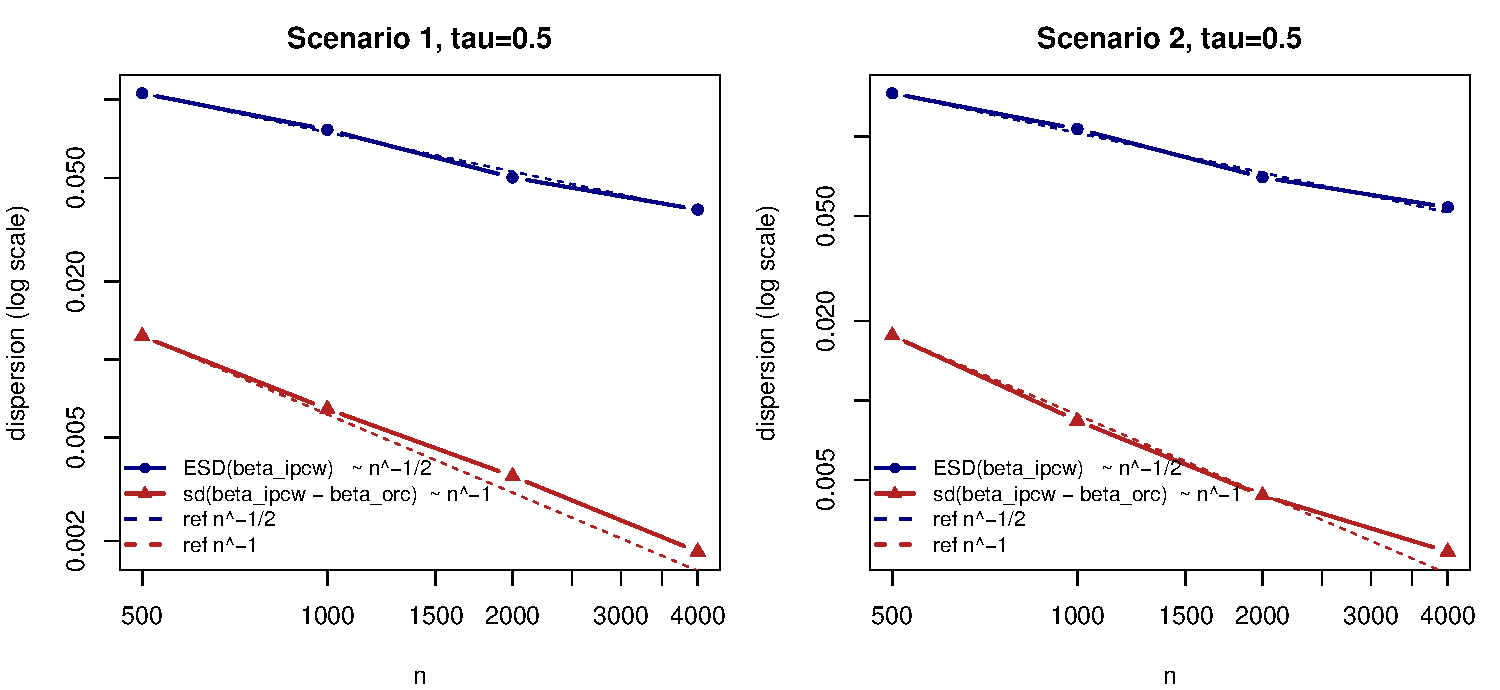
\includegraphics[width=0.62\textwidth]{../results/compare_rate.pdf}
\caption{Censoring-weight diagnostic. The estimated-vs-oracle weight gap (red;
fitted log--log slope near $-1$) shrinks faster than the estimator standard
deviation (blue, slope $\approx-1/2$), numerically supporting the second-order
($\chi^C=0$) censoring orthogonality of Lemma~\ref{lem:orth}.}
\label{fig:rate}
\end{figure}

\paragraph{Distributional features beyond the mean.} Under heteroscedasticity the
estimated quantile-trajectory surfaces $\widehat m_\tau(u,t)$ are non-parallel
across $\tau$, and $\widehat\bbeta_\tau$ recovers the analytic $\tau$-varying
covariate effect; point estimation is stable under heavy-tailed ($t_5$) and
right-skewed errors (Supplement~C). This is the regime a conditional-mean model
cannot describe and motivates the head-to-head comparison next.

\subsection{Comparison with the conditional-mean estimator of Sun et al.}\label{sec:suncmp}
We compare against the \emph{actual} estimator of \citet{sun2025semiparametric},
run from their published code (the compiled profile partial-likelihood slope
$\widehat\beta$ and their kernel baseline $\widehat\mu_0$), on a Sun-style
survival/truncation/fixed-visit design with a Sun-favorable Gamma
multiplicative-error marker, adapted to a binary group contrast. This is a
\emph{point-estimation} comparison ($R=500$ replicates; Monte-Carlo bias,
ESD and integrated mean-squared error (IMSE); no bootstrap). The conditional mean
is reconstructed from the fitted quantile process two ways: the model-free quantile
integral $\text{Q-INT}=\int_0^1 e^{Q_\tau}d\tau$ and the tail-stable
log-location-scale retransformation $\text{Q-LN}=\exp\{Q_{0.5}+\tfrac12\sigma^2\}$
(stronger than Sun's multiplicative-mean assumption; we report both). Five regimes
(Figure~\ref{fig:betatau}; Supplement Tables~C.6--C.8 give the full numbers):

\begin{figure}[t]\centering
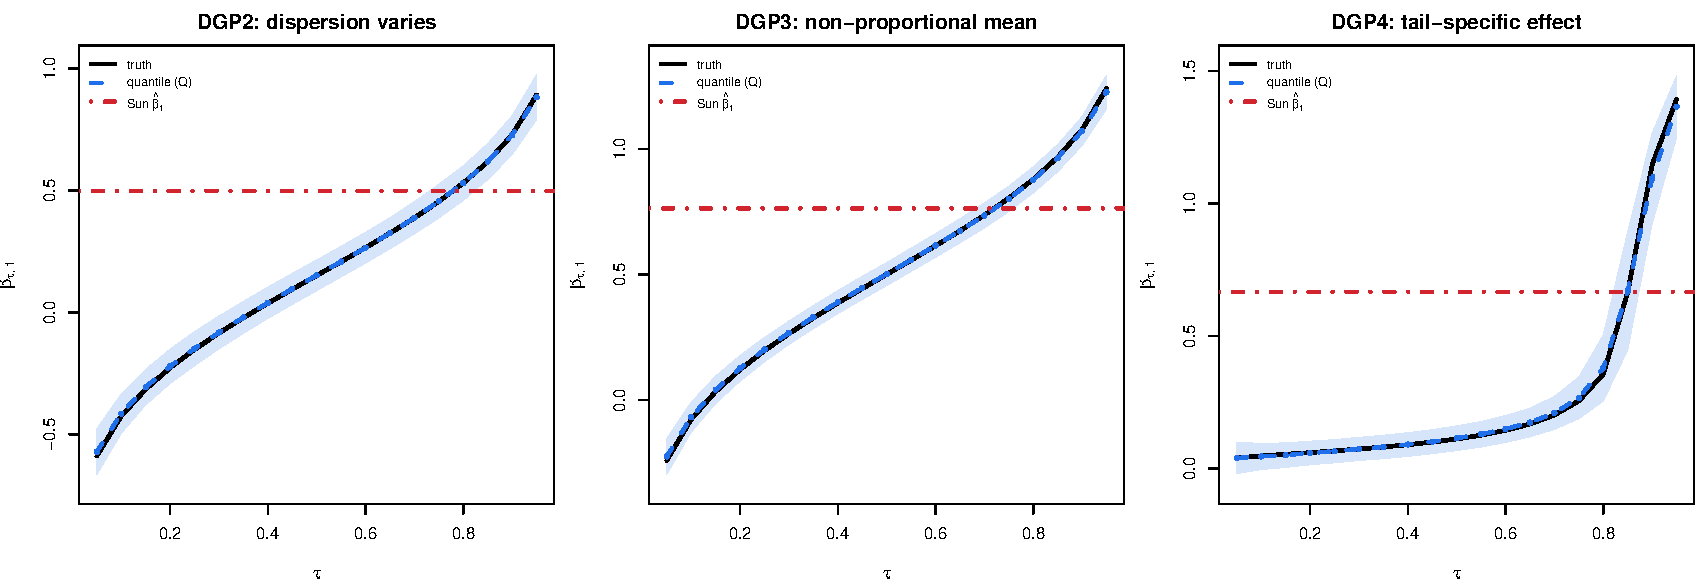
\includegraphics[width=\textwidth]{figs/cmp_betatau.pdf}
\caption{Covariate effect on the marker \emph{distribution}: true $\beta_{\tau,1}$
(solid) vs.\ our quantile-regression estimate (dashed, $\pm1$ Monte-Carlo SD band)
vs.\ Sun's single mean slope $\widehat\beta_1$ (flat dash-dot), $n=1000$. DGP2 the
mean is proportional yet the distributional effect varies with $\tau$; DGP3 the
effect varies and the mean contrast is non-proportional; DGP4 the effect is
confined to the upper tail. In each case the quantile estimate recovers the full
curve while the scalar mean coefficient collapses it to one number.}
\label{fig:betatau}
\end{figure}

\emph{DGP1 (proportional mean, Sun-favorable Gamma).} Both estimators are unbiased;
the mean and median slopes coincide, and the direct quantile slope has smaller
Monte-Carlo variability than the feasible Sun slope ($\sim$$4\times$ smaller ESD).
This is a point-estimation comparison, not an inferential-efficiency claim; an
oracle-$\alpha$ decomposition (Supplement~C) shows the difference is not due to
estimating the onset coefficient.
\emph{DGP2 (proportional mean, covariate-driven dispersion).} Sun's $\widehat\beta_1$
stays unbiased for the mean, but only the quantile slope reveals that the covariate
scales the spread ($\widehat\beta_{.75}-\widehat\beta_{.25}\approx0.6$).
\emph{DGP3 (non-proportional induced mean contrast --- the headline).} The mean
log-contrast $\Delta(u,t)$ truly varies over $(u,t)$, so no constant proportional
slope exists; Sun's basic slope collapses it to a pseudo-average and his fully
stratified Sec.~3.5 extension recovers the variation only at a large variance cost,
whereas the quantile reconstruction tracks $\Delta(u,t)$ with several-fold lower
IMSE (Figure~\ref{fig:contrast}).
\emph{DGP4 (tail-specific effect).} On the proportional mean target Sun is well
matched; the quantile method's value is \emph{detection}---it reveals the effect is
confined to a hidden upper-tail subgroup.
\emph{DGP5 (heavy-tailed error).} Under a $t_5$ log-error the conditional mean is
undefined, so this is an estimand-validity illustration, not a performance contest:
the quantile coefficients remain well-defined and stably estimated where the mean
target is ill-posed.

\begin{figure}[t]\centering
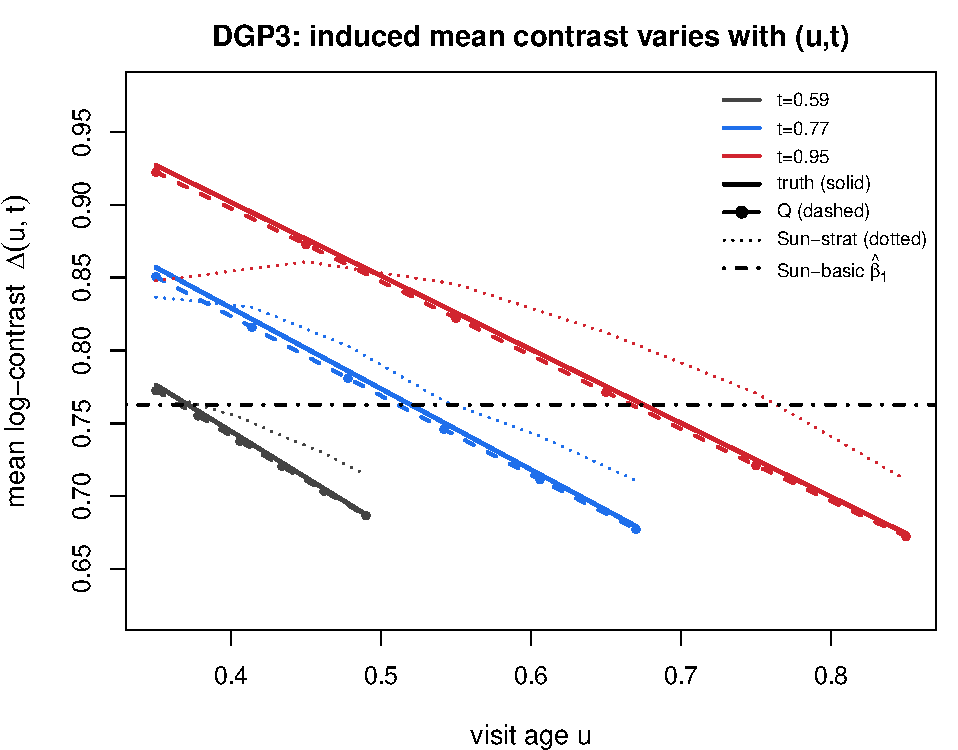
\includegraphics[width=0.6\textwidth]{figs/cmp_contrast.pdf}
\caption{DGP3 mean log-contrast $\Delta(u,t)=\log\{\E[Y|x_1{=}1]/\E[Y|x_1{=}0]\}$ at
three onset times, $n=1000$: truth (solid), quantile reconstruction (dashed), Sun's
basic proportional model (flat dash-dot), and his stratified-baseline extension
(dotted). The true contrast varies with $(u,t)$; the basic model collapses it to a
constant and the stratified extension is noisy, while the quantile reconstruction
tracks it.}
\label{fig:contrast}
\end{figure}

% ============================================================================
\section{Application: cortical thickness before amyloid positivity}\label{sec:app}

\editnote{Illustrative analysis on a synthetic ADNI-matched cohort; the real-data
analysis on ADNI is in preparation and will replace this section.}

We illustrate the method on a cohort matched to the Alzheimer's Disease
Neuroimaging Initiative (ADNI) design, in which a cortical-thickness biomarker is
tracked before the landmark of amyloid positivity. Participants are amyloid-negative
at staggered entry ages (delayed entry), are lost to follow-up, may die before
becoming amyloid-positive (competing event), and are imaged at irregular visits;
onset age $T^0$ is the age at first amyloid positivity. The covariates are an
\emph{APOE4} carrier indicator and sex. \emph{Because access to the curated cohort
is pending, the analysis below is run on a synthetic cohort generated to match the
ADNI sampling design (entry, truncation, censoring, competing death, visit process)
and serves to demonstrate the deliverables; it is not a substantive scientific
finding.}

We report, on the estimable interior region: (i) the median trajectory surface
$\widehat m_{0.5}(u,t)$; (ii) the carrier effect $\widehat\beta_{\tau,1}$ across
$\tau$ with subject-bootstrap bands, which answers whether \emph{APOE4} shifts the
lower tail of thickness (accelerated thinning in the already-vulnerable) more than
the median; and (iii) the induced mean contrast compared with the
\citet{sun2025semiparametric} mean coefficient, showing what the mean summary
misses (Figure~\ref{fig:app}). Sensitivity to the weighting (CC vs.\ IPCW), to the
inferential route (A-CV vs.\ B-OS-CF), and to crossing (handled by rearrangement of
predicted curves) is reported in Supplement~D.

\begin{figure}[t]\centering
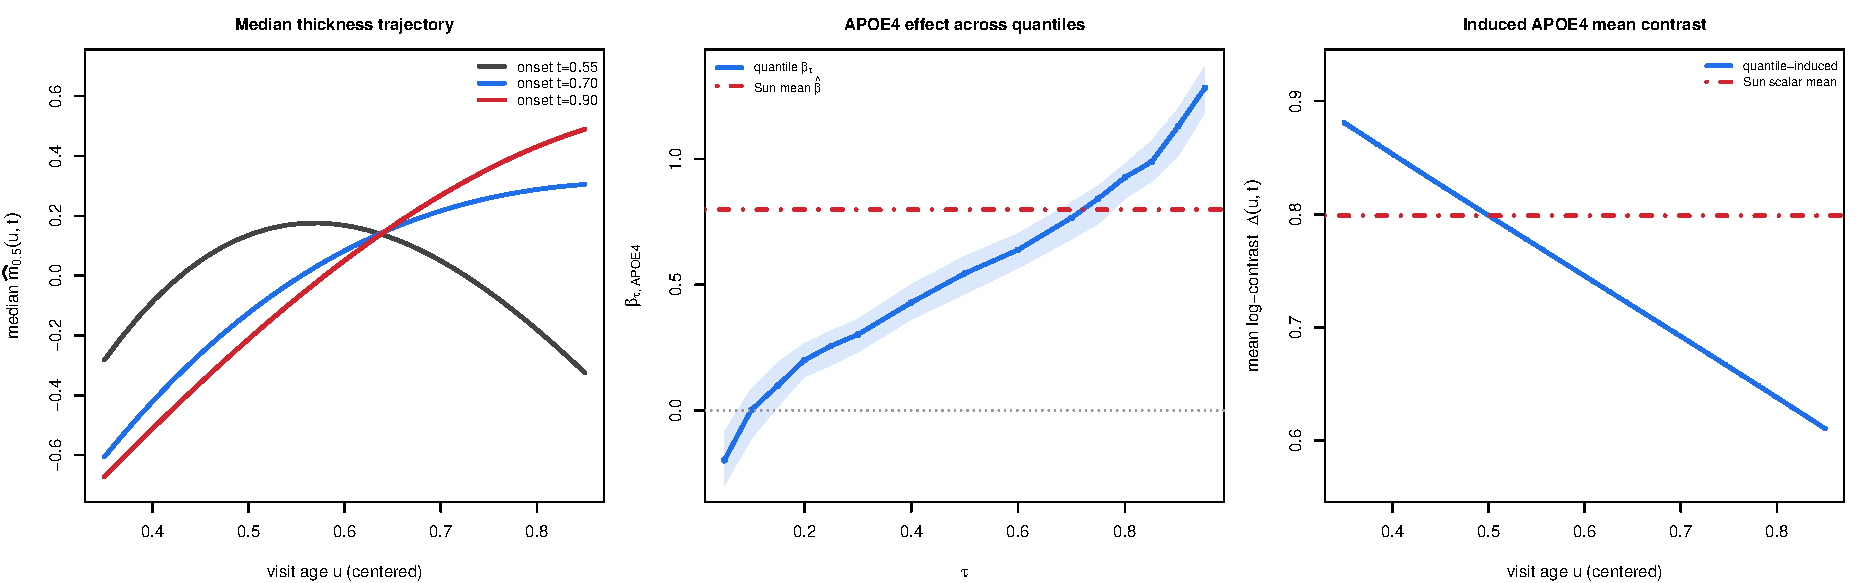
\includegraphics[width=\textwidth]{figs/app_panels.pdf}
\caption{Illustrative analysis on a synthetic ADNI-matched cohort. Left: estimated
median thickness trajectory $\widehat m_{0.5}(u,t)$ over visit age $u$ at three
onset ages $t$. Center: \emph{APOE4} carrier effect $\widehat\beta_{\tau,1}$ across
$\tau$ with $95\%$ subject-bootstrap band; a non-flat curve indicates a
distributional (not pure location) effect. Right: induced mean log-contrast from
the quantile fit (curve) vs.\ the scalar conditional-mean coefficient (flat line).
Synthetic data; for illustration of the outputs only.}
\label{fig:app}
\end{figure}

% ============================================================================
\section{Discussion}\label{sec:disc}

We have introduced an event-aligned conditional quantile trajectory model for a
biomarker observed before disease onset under left truncation, right censoring,
competing death, and irregular visits, identified it without modeling the onset or
censoring mechanisms, and given an orthogonal, cross-fitted one-step estimator with
$\sqrt n$ inference. The conditional median effect $\beta_{0.5}$ is a location
effect on the log-marker and need not equal the multiplicative mean coefficient of
\citet{sun2025semiparametric} under heteroscedasticity. Against their actual
estimator, the comparison is not that we estimate the mean better: when the
proportional mean holds both are unbiased. The contribution is that the quantile
family answers questions the mean model structurally cannot---covariate-driven
dispersion, non-proportional induced mean contrasts, and tail-specific
effects---and remains well-defined where heavy tails make the conditional mean
ill-posed.

Robustness to the onset-time distribution (including non-proportional-hazards and
accelerated-failure-time onset) is intrinsic to the conditional formulation, since
the onset mechanism is never modeled. Genuine extensions include interval-censored
or latent onset $T^0\in(L,R]$, informative onset ascertainment, marginalization
over $T^0$, and informative visit processes (which reintroduce a visit weight). A
complete root-$n$ theory for the cross-validated joint-sieve estimator and a
bootstrap consistency proof remain open and are natural next steps.

\bibliographystyle{plainnat}
\bibliography{mwqtm_references}

\end{document}
